\chapter{Results}

We have tested our algorithm on wide range of input skeletons.
The input skeletons varied in number of branch, leaf, and connection nodes.
The quality of generated base manifold mesh is independent from the number of branch, leaf, and connection nodes.
Likewise, the number of nodes connected to a branch node does not affect the quality of generated base mesh.
Base meshes generated with our algorithm have good edge flow.
That means faces of our base meshes are aligned with bones of their corresponding input skeleton.
Thanks to the good edge flow base meshes produced by our algorithm can be animated using the input skeleton.
Rigging weights are computed naturally because each vertex is affected by exactly two nodes in the input skeleton.
Base meshes are composed mainly from quadrilateral faces.
Triangular faces are present only at leaf nodes.

\section{Humanoids, animals, plants and bugs}

The SQM algorithm was designed to model real life objects like animals, humanoids, and bugs.
Because of that our set of test skeletons is resembling these real life objects.
The generated base meshes capture the geometry represented by the input skeleton.
A goat creature generated by our algorithm is shown in Figure \ref{fig:result_goat}.
During our testing we have found that the number of neighbours of a branch node does not affect the quality of resulting base mesh.
However, we have also found that the distribution of branch node neighbours does affect the quality of resulting base mesh.
In Figure \ref{fig:pavuk_skl_1} an input skeleton of a spider is defined.
After our base mesh algorithm is executed a base mesh shown in Figure \ref{fig:pavuk_mesh_1} is generated.
The generated base mesh does not resemble the desired output.
This is caused by the triangulation step.
The intersection vertices forming spiders body are not approximating a polyhedron.
The triangulation does not fail but splits spiders legs in two groups connected to spiders top and bottom.
In order to recover from this situation we need to introduce additional nodes into the input skeleton.
In order to better approximate spiders body we have placed the additional nodes on the top and bottom of its body.
The updated skeleton is shown in Figure \ref{fig:pavuk_skl_2}.
The generated base mesh from the new skeleton is shown in Figure \ref{fig:pavuk_mesh_2}.
The generated base mesh now better resembles the desired output.
However, new triangular faces were introduced into the skeleton.
Plants, humanoids and animals do not produce this kind of artifacts.
This is mainly due to their skeletal structure.
Branch nodes in their skeletons usually have better distribution of neighbours which means their branch nodes better approximate polyhedrons.

\begin{figure}
        \centering
        \begin{subfigure}[b]{0.4\textwidth}
        	\centering
                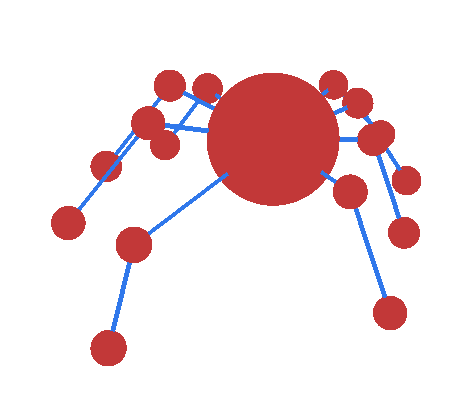
\includegraphics[width=\textwidth]{images/pavuk_kostra.png}
                \caption{Original spider input skeleton.}
                \label{fig:pavuk_skl_1}
        \end{subfigure}%
        ~ %add desired spacing between images, e. g. ~, \quad, \qquad etc.
          %(or a blank line to force the subfigure onto a new line)
        \begin{subfigure}[b]{0.4\textwidth}
        	\centering
                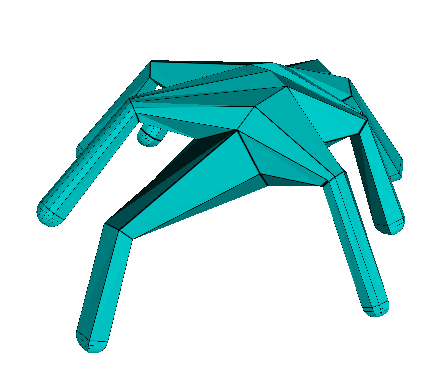
\includegraphics[width=\textwidth]{images/pavuk_fail.png}
                \caption{Base mesh from original skeleton with undesired mesh topology.}
                \label{fig:pavuk_mesh_1}
        \end{subfigure}
        \\ %add desired spacing between images, e. g. ~, \quad, \qquad etc.
          %(or a blank line to force the subfigure onto a new line)
        \begin{subfigure}[b]{0.4\textwidth}
        	\centering
                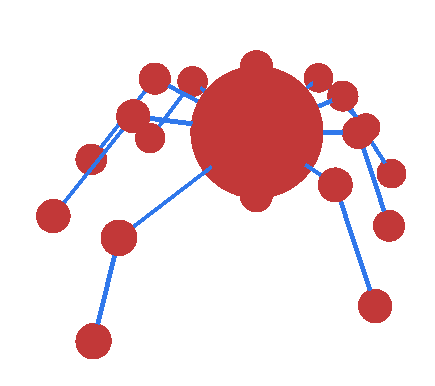
\includegraphics[width=\textwidth]{images/pavuk_kostra_upravena.png}
                \caption{Changed input skeleton to allow better triangulation.}
                \label{fig:pavuk_skl_2}
        \end{subfigure}
        ~ %add desired spacing between images, e. g. ~, \quad, \qquad etc.
          %(or a blank line to force the subfigure onto a new line)
        \begin{subfigure}[b]{0.4\textwidth}
        	\centering
                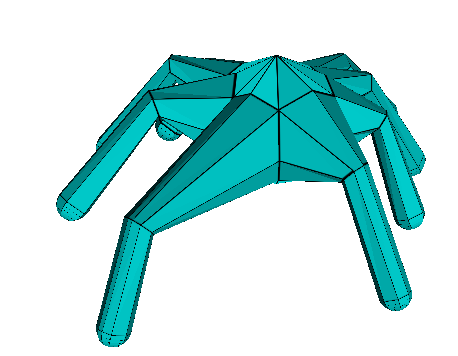
\includegraphics[width=\textwidth]{images/pavuk_dobry.png}
                \caption{Final base mesh with extra triangular faces but acceptable mesh topology.}
                \label{fig:pavuk_mesh_2}
        \end{subfigure}
        \caption[Base mesh of a spider]{Base mesh of a spider.}\label{fig:pavuk}
\end{figure}

\begin{figure}
    \centering
    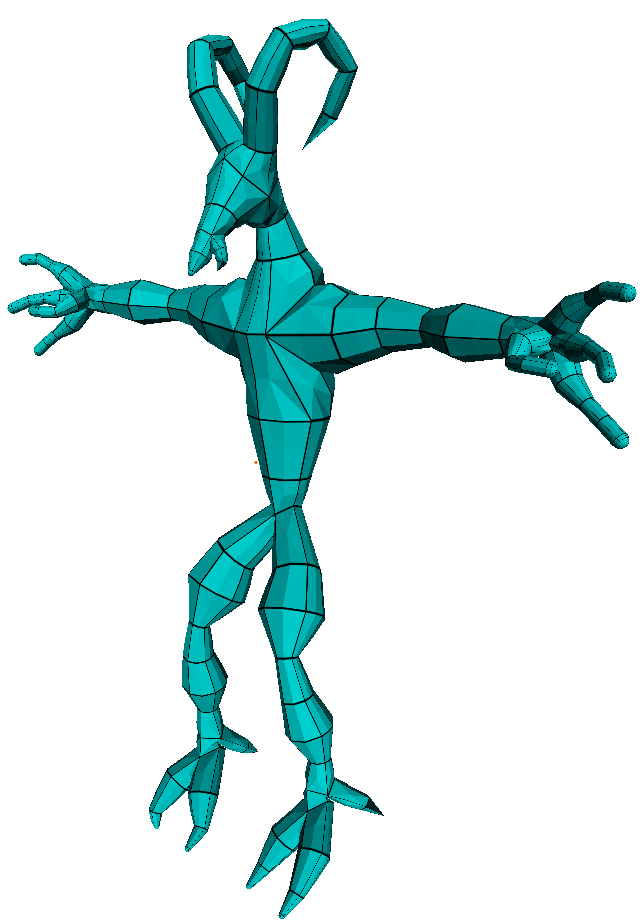
\includegraphics[width=\textwidth]{images/goat_1.png}
    \caption[Generated goat creature]{Goat creature generated with our algorithm. The input skeleton has 150 nodes. The node distribution is 9 branch nodes, 123 connection nodes, and 18 leaf nodes. Generated mesh consists of 1061 vertices and 1126 faces. The mesh was generated in 0.074 s. The displayed mesh is tessellated with tessellation factor 2.}
    \label{fig:result_goat}
\end{figure}

\section{Linear and cyclic skeletons}

Linear and cyclic skeleton base mesh generation was introduced in this thesis.
Base meshes from linear skeletons without branching produce expected results.
Meshes produced by our algorithm have good edge flow and produce triangular faces only at the begging and end of the generated mesh.
The additional parameter setting the number of vertices for each node of a linear skeletons does not decrease the robustness of our approach.
Because with tessellation it is negligible.
A linear skeleton is shown in Figure \ref{fig:lin_skl} and generated base mesh in Figure \ref{fig:lin_mesh}.
In fact, with tessellation the mesh can be generated faster with the minimal number of vertices and still produce visual results equivalent to more complex meshes.
Generation of base meshes from cyclic skeletons produces good results.
The cycle can be at arbitrary place in the input skeleton.
Base meshes with various genus can be generated.
However, the faces bridging cyclic nodes are connected solely with triangular faces.
This is because the valency of both one rings is not always equal.
Some of the triangular faces could be merged into quadrilaterals in a post-process similar to the one used in B-Mesh \cite{ji_bm}.
A cyclic input skeleton is shown in Figure \ref{fig:cyclic_skl} and its corresponding base mesh generated by our algorithm in Figure \ref{fig:cyclic_mesh}.

\begin{figure}[h]
        \centering
        \begin{subfigure}[b]{0.4\textwidth}
        	\centering
                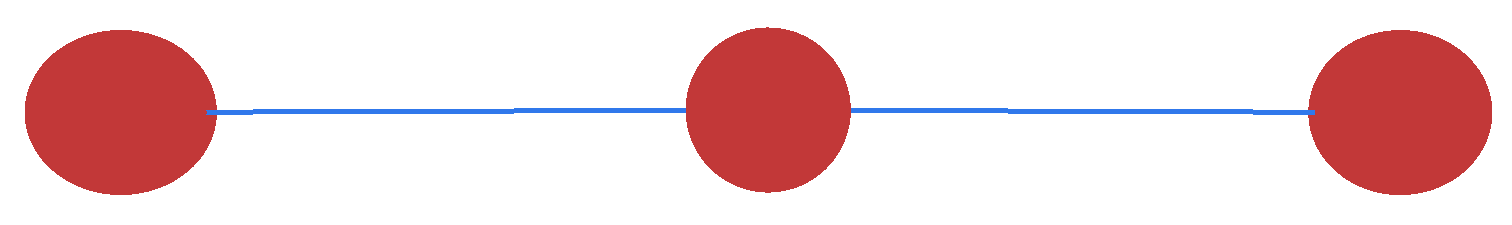
\includegraphics[width=\textwidth]{images/cerv_skl.png}
                \caption{Linear skeleton.}
                \label{fig:lin_skl}
        \end{subfigure}%
        \qquad %add desired spacing between images, e. g. ~, \quad, \qquad etc.
          %(or a blank line to force the subfigure onto a new line)
        \begin{subfigure}[b]{0.4\textwidth}
        	\centering
                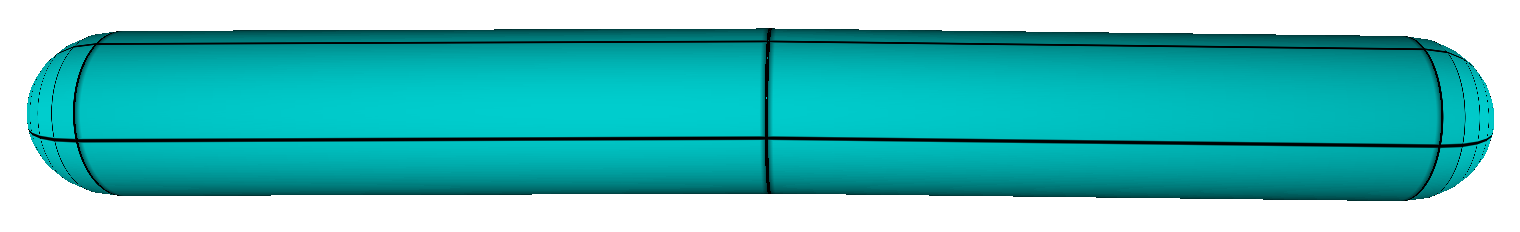
\includegraphics[width=\textwidth]{images/cerv_mesh.png}
                \caption{Tessellated linear base mesh.}
                \label{fig:lin_mesh}
        \end{subfigure}%
        \\ %add desired spacing between images, e. g. ~, \quad, \qquad etc.
          %(or a blank line to force the subfigure onto a new line)
        \begin{subfigure}[b]{0.5\textwidth}
        	\centering
                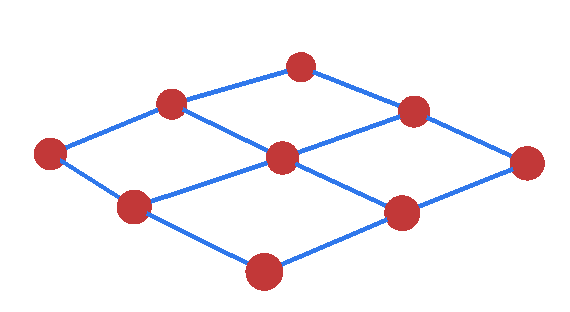
\includegraphics[width=\textwidth]{images/cycle_skl.png}
                \caption{Cyclic skeleton.}
                \label{fig:cyclic_skl}
        \end{subfigure}%
        ~ %add desired spacing between images, e. g. ~, \quad, \qquad etc.
          %(or a blank line to force the subfigure onto a new line)
        \begin{subfigure}[b]{0.5\textwidth}
        	\centering
                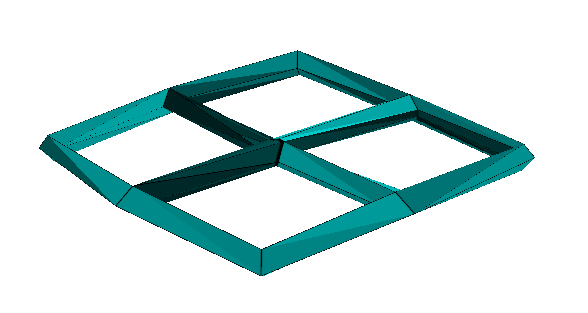
\includegraphics[width=\textwidth]{images/cycle_mesh.png}
                \caption{Base mesh with genus four.}
                \label{fig:cyclic_mesh}
        \end{subfigure}
        \caption[Cyclic and linear base meshes]{Cyclic and linear base meshes.}\label{fig:pavuk}
\end{figure}

\section{Capsules, ellipsoid nodes and tessellation}

Capsules are automatically generated at leaf nodes.
The generated capsules can be naturally tessellated with our existing pipeline.
The number of nodes inserted into the input skeleton to form a capsule is currently automatically computed from the radius of a capsule node.
The automatic approach produces visually plausible capsules, especially when the generated base mesh is tessellated.
A capsule is shown in Figure \ref{fig:caps}.

Ellipsoid nodes can be defined as connection or branch nodes.
The generation of ellipsoid capsules is not yet supported.
Generated ellipsoid approximate the volume of the input skeleton.
Ellipsoid nodes can also be used to smooth sharp angles between two skeletal bones.
A slightly rotated sphere can produce better edge flow.
Ellipsoid nodes were used to generate fish in Figure \ref{fig:fish}.

Tessellation is used to increase the visual quality of generated base mesh in real time on GPU.
After tessellation the generated base mesh closely approximates the input skeleton.
However, the tessellated mesh can self intersect.
This is mainly caused by the original input skeleton.
We attempted to solve this automatically without forcing the artist to edit the input skeleton by introducing radius scaling reduction.
Our radius scaling method helped with various self-intersecting meshes.
But certain meshes were still preferable to edit manually.
Generated base mesh is shown in Figure \ref{fig:no_tess}.
After tessellation the base mesh is shown in Figure \ref{fig:tess}.

\begin{figure}[h]
        \centering
        \begin{subfigure}[b]{0.25\textwidth}
        	\centering
                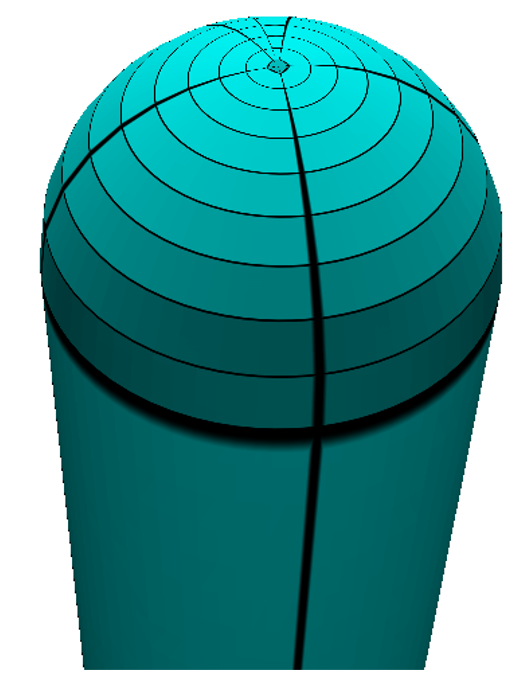
\includegraphics[height=\textwidth]{images/capsule.png}
                \caption{Leaf node capsule.}
                \label{fig:caps}
        \end{subfigure}%
        \qquad %add desired spacing between images, e. g. ~, \quad, \qquad etc.
          %(or a blank line to force the subfigure onto a new line)
        \begin{subfigure}[b]{0.4\textwidth}
        	\centering
                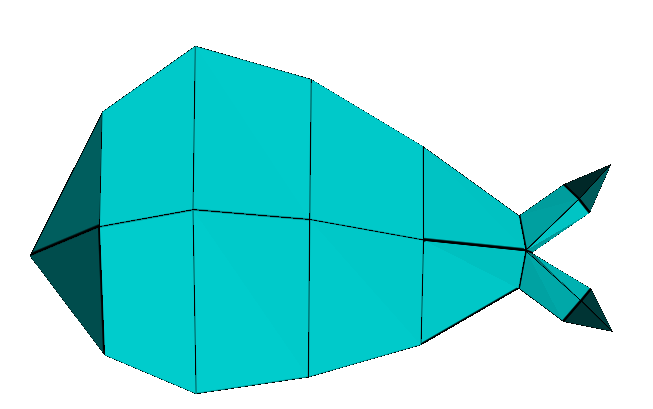
\includegraphics[width=\textwidth]{images/ryba_mesh.png}
                \caption{Fish with ellipsoid nodes.}
                \label{fig:fish}
        \end{subfigure}
        \caption[Capsules and ellipsoid nodes]{Capsules and ellipsoid nodes.}\label{fig:caps_ell}
\end{figure}

\begin{figure}[h]
        \centering
        \begin{subfigure}[b]{0.4\textwidth}
        	\centering
                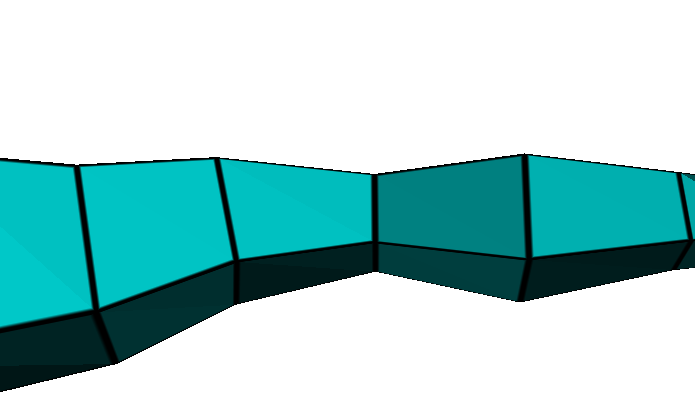
\includegraphics[width=0.8\textwidth]{images/not_tessellated_mesh.png}
                \caption{Not tessellated mesh.}
                \label{fig:no_tess}
        \end{subfigure}
        \qquad %add desired spacing between images, e. g. ~, \quad, \qquad etc.
          %(or a blank line to force the subfigure onto a new line)
        \begin{subfigure}[b]{0.4\textwidth}
        	\centering
                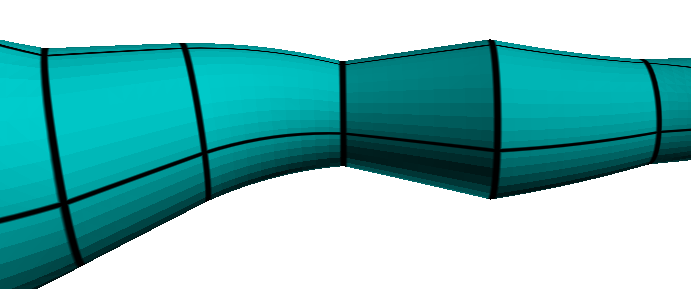
\includegraphics[width=0.8\textwidth]{images/tessellated_mesh.png}
                \caption{Tessellated mesh.}
                \label{fig:tess}
        \end{subfigure}
        \caption[Tessellation results]{Tessellation results.}\label{fig:tes_notess}
\end{figure}

\section{Comparison with SQM algorithm}

Our algorithm is also capable of generating base meshes from skeletons on which SQM would fail.
For example in Figure \ref{fig:comp_eel} we can see a fish as would be produced by SQM without ellipsoid nodes.
The generated base mesh resembles an eel.
Our algorithm with ellipsoid nodes Figure \ref{fig:comp_fish} produces a base mesh that corresponds to a fish.
In Figure \ref{fig:comp_cycle} we can see a cyclic mesh generated by our algorithm.
Producing a similar mesh in SQM is not possible as the cycles do not lie in symmetrical region of the input skeleton and SQM would not close them.
Figure \ref{fig:comp_cycle_sqm} shows base mesh from asymmetric cyclic skeleton as would be generated by SQM.

\begin{figure}[ht]
        \centering
        \begin{subfigure}[b]{0.45\textwidth}
        	\centering
			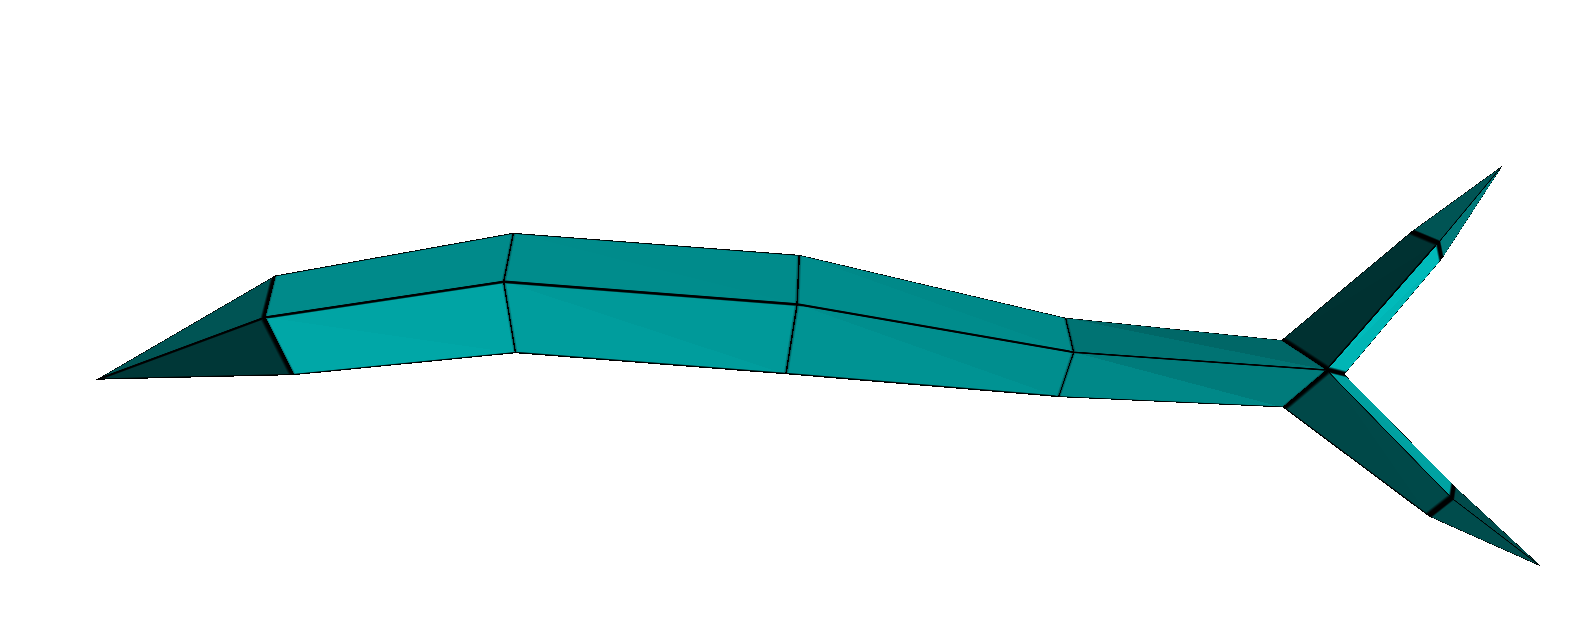
\includegraphics[width=0.8\textwidth]{images/ryba_no_elips}
            \caption{Fish without ellipsoid nodes as would be generated by SQM.}
            \label{fig:comp_eel}
        \end{subfigure}%
        ~ %add desired spacing between images, e. g. ~, \quad, \qquad etc.
          %(or a blank line to force the subfigure onto a new line)
        \begin{subfigure}[b]{0.45\textwidth}
        	\centering
			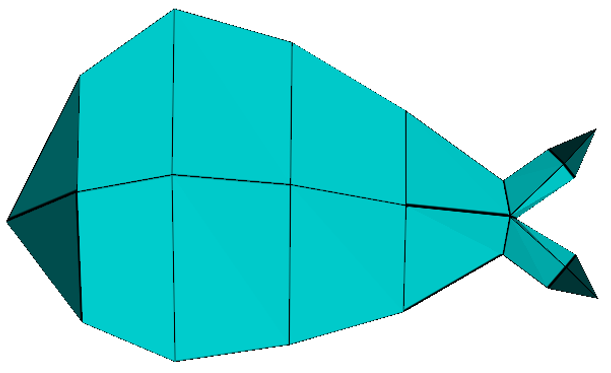
\includegraphics[width=0.7\textwidth]{images/ellipsoid_fish_ilu_2}
            \caption{Fish with ellipsoid nodes generated by our algorithm.}
            \label{fig:comp_fish}
        \end{subfigure}
        \\ %add desired spacing between images, e. g. ~, \quad, \qquad etc.
          %(or a blank line to force the subfigure onto a new line)
        \begin{subfigure}[b]{0.45\textwidth}
        	\centering
			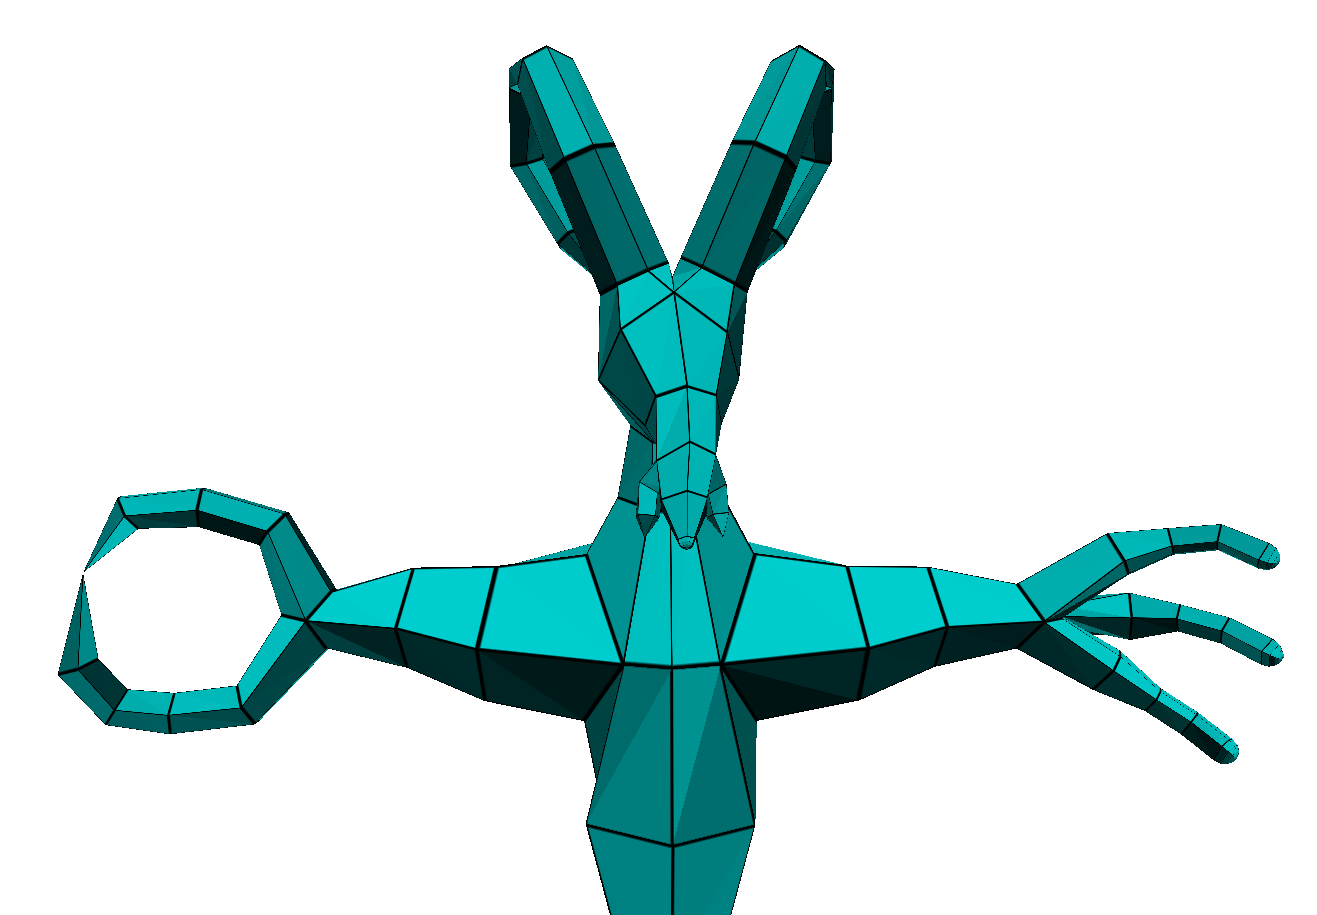
\includegraphics[width=0.9\textwidth]{images/goat_amput_sqm_3}
            \caption{Mesh from cyclic skeleton as would be generated by SQM.}
            \label{fig:comp_cycle_sqm}
        \end{subfigure}
        ~ %add desired spacing between images, e. g. ~, \quad, \qquad etc.
          %(or a blank line to force the subfigure onto a new line)
        \begin{subfigure}[b]{0.45\textwidth}
        	\centering
			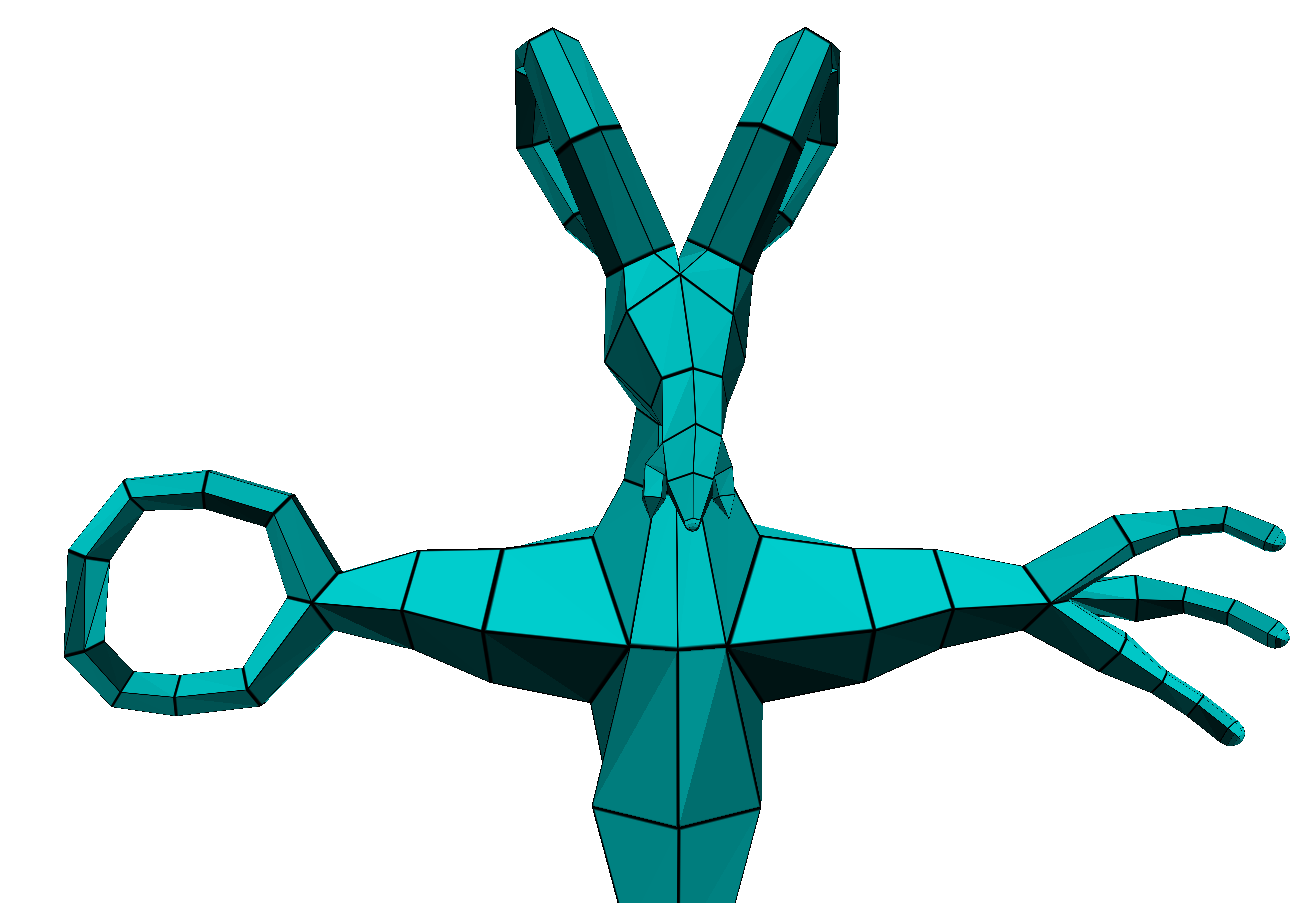
\includegraphics[width=0.9\textwidth]{images/goat_amput_3}
            \caption{Mesh from cyclic skeleton generated by our algorithm.}
            \label{fig:comp_cycle}
        \end{subfigure}
        \caption{Comparision of SQM (left) to our implementation (right).}
        \label{fig:comp_ilu}
\end{figure}

\section{Computation time}

In Table \ref{tab:models} we show the details about measured models.
For each model its total number of nodes as well as node distribution is shown.
Table \ref{tab:results} shows how much time each stage of our base manifold mesh algorithm takes.
Time was measured on Intel\textsuperscript{\textregistered}  Core\textsuperscript{TM} i7-3615QM a four core processor with each core clocked at 2.3 GHz.
Time is measured in milliseconds.
From the table we can see that the joining step, during which the tubular structure is generated, took the most time.
Therefore, it is a candidate for optimization since other steps of the algorithm took nearly no time to execute.
However, even at current speed we can generate base meshes at interactive frame rate.
For example, the goat creature shown in Figure \ref{fig:result_goat} can be generated 13.5 times per second.
From the tables we can also conclude that computation time is also highly dependant on the number of branch nodes and their number of neighbours.
For example, a dummy consisting of 140 nodes is computed in 57 milliseconds.
On the other hand a goat creature with 150 nodes is computed in 74 milliseconds.

BNP generation and subdivision steps are dependant on the number of branch nodes and number of neighbours of each branch node.
The more neighbours a node has the longer it takes to execute the triangulation.
The BNP joining step is limited by our used data structure.

%At each step of the algorithm the only prerequisite is that the parent of current node has been processed.
%We can exploit this fact and compute each child of a branch node in a parallel thread in order to increase the overall computation speed.
%If we want to increase the speed of computation with parallel joining of nodes we would need a half-edge data structure supporting parallel addition of vertices and edges.

\begin{table}[h]
\centering
\begin{tabular}{l|ccc||c}\hline
\multicolumn{1}{c}{\textbf{Model}} & \multicolumn{4}{c}{\textbf{Node Distribution}} \\
   & \#branch & \#connection & \#leaf & \textbf{\#nodes} \\ \hline
  worm & 21 & 2 & 0 & 23 \\
  dummy & 2 & 49 & 5 & 56 \\
  cycle & 1 & 12 & 1 & 14 \\
  octopus & 1 & 117 & 13 & 131 \\
  dummy 2 & 5 & 122 & 13 & 140 \\
  goat & 9 & 123 & 18 & 150 \\
  tree & 18 & 129 & 24 & 171 \\ \hline
\end{tabular}
\caption[Table show statics of input skeletons]{Table show statics of input skeletons. From left to right: name of the model, number of branch nodes, number of connection nodes, number of leaf nodes, and total number of nodes.}
\label{tab:models}
\end{table}

\begin{table}[h]
\centering
\begin{tabular}{l|cccc||c}\hline
\multicolumn{1}{c}{\textbf{Model}} & \multicolumn{5}{c}{\textbf{Timing of steps in computer clicks}} \\
   & straightening & generation & subdivision & joining & \textbf{Total} \\ \hline
  worm & 0 & 0 & 0 & 5 & 5 \\
  dummy & 0 & 4 & 2 & 15 & 21 \\
  cycle & 0 & 4 & 2 & 18 & 24 \\
  octopus & 1 & 9 & 5 & 54 & 69 \\
  dummy 2 & 1 & 11 & 6 & 39 & 57 \\
  goat & 1 & 16 & 10 & 47 & 74 \\
  tree & 3 & 28 & 15 & 50 & 96 \\ \hline
\end{tabular}
\caption[Table show statics of base mesh algorithm]{Table show statics of base mesh algorithm. From left to right: name of the model, timing of each step of the algorithm measured in milliseconds.}
\label{tab:results}
\end{table}